\documentclass[letterpaper]{article}
\usepackage[utf8]{inputenc}
\usepackage[T1]{fontenc}
\usepackage[activeacute,english]{babel}
\usepackage[vmargin=4cm,tmargin=3cm,hmargin=2cm,letterpaper]{geometry}%
\usepackage{helvet}
\usepackage{amsmath,amsfonts,amssymb}
\usepackage{graphicx}
\usepackage{color}
\usepackage{xcolor}
\usepackage{verbatim}
\usepackage{tabls}
\usepackage{lastpage}
\usepackage{fancyhdr}
\usepackage{url}
\usepackage{listings}
\usepackage{tikz}
\usepackage{pgf}
\usepackage{pgffor}
\usepgfmodule{plot}
\usepackage{wrapfig}
\usepackage{ifpdf}
\usepackage{amssymb}
\usepackage{pifont}
\usepackage{epstopdf}
\usepackage{graphicx} % Allows including images
\usepackage{booktabs} % Allows the use of \toprule, \midrule and \bottomrule in tables
\usepackage{tikz}
\usetikzlibrary{arrows,decorations,snakes,backgrounds,fit,calc,through,scopes,positioning,automata,chains,er,fadings,calendar,matrix,mindmap,folding,patterns,petri,plothandlers,plotmarks,shadows,shapes,shapes.arrows,topaths,trees}

\lstset{% general command to set parameter(s)
%   basicstyle=\small,
  % print whole listing small
%   keywordstyle=\color{black}\bfseries\underbar,
  % underlined bold black keywords
%   identifierstyle=,
  % nothing happens
%   commentstyle=\color{white}, % white comments
%   stringstyle=\ttfamily,
  % typewriter type for strings
  showstringspaces=false}
  % no special string spaces

\pagestyle{fancy}
\color{black}
\fancyhead{}
\renewcommand{\headrule}{\hrule\vspace*{0.5mm}\rule{\linewidth}{0.8mm}}
\renewcommand{\familydefault}{\sfdefault}

\graphicspath{{./images/}}
\lhead{
\includegraphics[width=2cm]{logoucr.png}}
\rhead{
\includegraphics[width=3cm]{eie-text-gray-6x3cm.png}}
\chead{UNIVERSIDAD DE COSTA RICA\\FACULTAD DE INGENIERÍA\\ESCUELA DE INGENIERÍA ELÉCTRICA\\\textbf{ESTRUCTURAS ABSTRACTAS DE DATOS Y\\ ALGORITMOS PARA INGENIERÍA}\\IE-0217\\I CICLO 2014\\PROPUESTA DEL PROYECTO DE ESTRUCTURAS DE DATOS}

\lfoot{}%
\cfoot{}%
%\cfoot{\thepage\ de \pageref{LastPage}}%
\rfoot{}%

%%%%%%%%%%%%%%%%%%%%%%%%%%%%%%%%%%%%%%%%%%%%%%%%%%%%%%%%%%%%%%%%%%%%%%%%%%%%%%%%%%%%%%%%%%%%%%%%%%%%%%%%%%%%%%%
\newcommand{\uic}{blue} %user-input color
%%%%%%%%%%%%%%%%%%%%%%%%%%%%%%%%%%%%%%%%%%%%%%%%%%%%%%%%%%%%%%%%%%%%%%%%%%%%%%%%%%%%%%%%%%%%%%%%%%%%%%%%%%%%%%%%%%
\newcommand{\uim}{\_\_} %user-input marker
%%%%%%%%%%%%%%%%%%%%%%%%%%%%%%%%%%%%%%%%%%%%%%%%%%%%%%%%%%%%%%%%%%%%%%%%%%%%%%%%%%%%%%%%%%%%%%%%%%%%%%%%%%%%%%%%%%
\newcommand{\userinput}[1]{\textcolor{\uic}{\uim#1\uim}}


%%%%%%%%%%%%%%%%%%%%%%%%%%%%%%%%%%%%%%%%%%%%%%%%%%%%%%%%%%%%%%%%%%%%%%%%%%%%%%%%%%%%%%%%%%%%%%%%%%%%%%%%%%%%%%%%%%
\begin{document}\vspace*{2cm}
%%%%%%%%%%%%%%%%%%%%%%%%%%%%%%%%%%%%%%%%%%%%%%%%%%%%%%%%%%%%%%%%%%%%%%%%%%%%%%%%%%%%%%%%%%%%%%%%%%%%%%%%%%%%%%%%%%

%%%%%%%%%%%%%%%%%%%%%%%%%%%%%%%%%%%%%%%%%%%%%%%%%%%%%%%%%%%%%%%%%%%%%%%%%%%%%%%%%%%%%%%%%%%%%%%%%%%%%%%%%%%%%%%%%%
\begin{center}
\Huge
\textbf{Data Structures Implementations for K-Da Library}
\vspace*{1cm}
\end{center}

\noindent
\small\baselineskip=14pt
\textbf{Estudiantes:} \\
\text{David Pérez Bolaños - B04769}\\
\text{Andrey Pérez Salazar - B25084}\\
\text{Andrés Sánchez López - B26214}\\


\begin{figure}[ht]
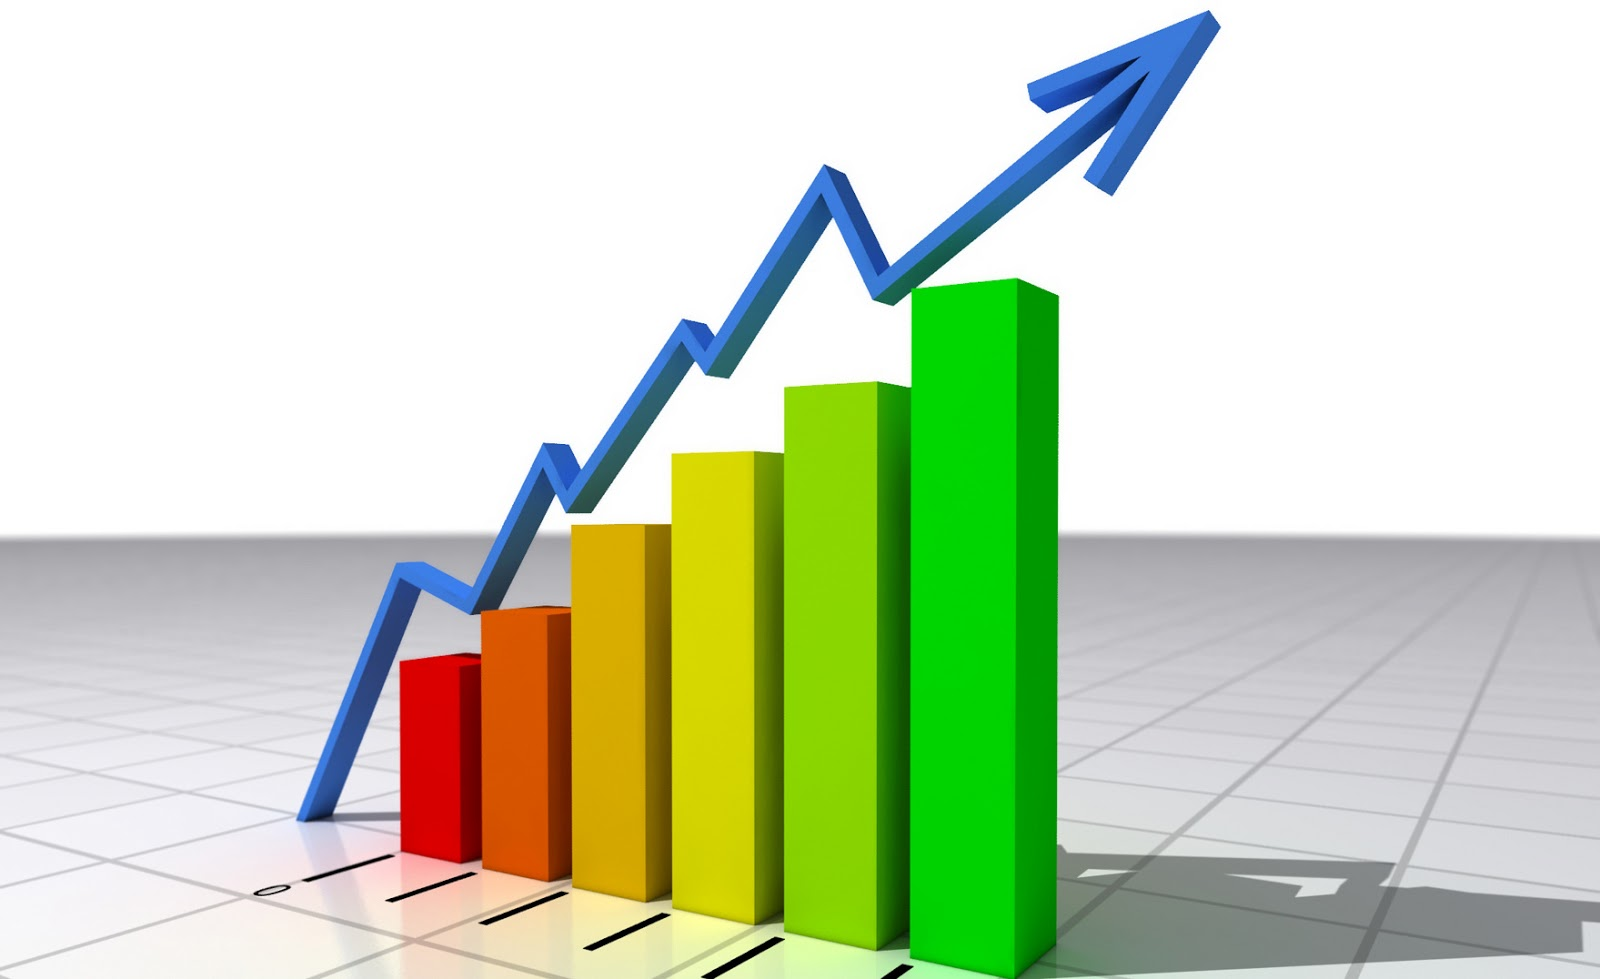
\includegraphics[width=1\linewidth]{ese.jpg}
\end{figure}


%%%%%%%%%%%%%%%%%%%%%%%%%%%%%%%%%%%%%%%%%%%%%%%%%%%%%%%%%%%%%%%%%%%%%%%%%%%%%%%%%%%%%%%%%%%%%%%%%%%%%%%%%%%%%%%%%%
\section{Introducción}
\hyphenation{fun-cio-na-li-dad}
\quad \quad La creación de librerías en lenguajes de programación ayuda a generar una interfaz bien definida para una cierta funcionalidad en específico, es decir,
dan al usuario ciertas ventajas a la hora de programar de una manera sencilla. Estas también sirven para separar por módulos un programa y de esta manera generar un código más claro y ordenado.\\

Una librería es un conjunto de funciones utilizadas para desarrollar software, no son programas, pero por lo general si son utilizadas por los programas 
para poder funcionar de forma correcta; el desarrollo de librerías sirve como apoyo a los programadores para tener más facilidades en la implementación de código
en sus programas y a contar con más recursos para realizar sus proyectos. Existen muchas librerías para los diferentes lenguajes informáticos que hay.\\

En este caso, se implementó una librería cuya función es comparar los movimientos entre dos personas. Nuestra librería esta programada
en el lenguaje C++. La idea de esta librería fue crear métodos o funciones en código, e implementar diferentes herramientas como el Kinect y el lenguaje informático Processing para
lograr la función principal: comparar los movimientos de dos personas, esto, de manera virtual; esta técnica de comparación de movimientos humanos se utiliza mucho 
en videojuegos, efectos especiales, medicina, simuladores, entre otros.\\

Para continuar con el desarrollo del proyecto, se desarrollaron los siguientes objetivos: la implementación de algunas estructuras de datos, esto, en la manipulación de información obtenida mediante el Kinect de manera que se quiere realizar un análisis implementando algunas de ellas, para así determinar y comparar, qué estructuras son las más eficientes a la hora de manipular esta información.\\

En general, las estructuras de datos implementarán las funciones básicas de acceso o búsqueda de datos, lo cual nos ayudará a tener un manejo más rápido y ordenado de los datos obtenidos por el Kinect.

%%%%%%%%%%%%%%%%%%%%%%%%%%%%%%%%%%%%%%%%%%%%%%%%%%%%%%%%%%%%%%%%%%%%%%%%%%%%%%%%%%%%%%%%%%%%%%%%%%%%%%%%%%%%%%%%%%
\section{Desarrollo}

\subsection{K-Da Library}

\quad \quad Como se mencionó con anterioridad, la creación de librerías de programación corresponden a una funcionalidad en específico. En nuestro caso, la librería
implementada corresponde a un conjunto de métodos computacionales para llevar a cabo la comparación de movimientos. Para lograr esto, se implementó 
la librería en lenguaje C++, sin embargo, los datos de los movimientos son tomados de un controlador de juego libre y entretenimiento llamado Kinect; creado por Alex Kipman, desarrollado por Microsoft para la videoconsola
Xbox 360 y OpenNI, que es el software utilizado para reproducir una interfaz en las computadoras, de las imágenes que recibe el Kinect de donde toma los datos. De este software se hablará detallamente más adelante. 
Además se usa también el lenguaje de programación Processing para poder obtener del Kinect los datos que se produzcan. Relacionadas estas cuatro importantes
herramientas es que nuestra librería da el funcionamiento esperado. 

\subsection{Funcionamiento de K-Da Library}

\quad \quad Retomando las herramientas que forman parte de la librería, iniciamos este apartado para describir, de una manera general, como se da la comparación de los movimientos.

\subsubsection{Código en C++}

\quad \quad El código de la librería fue desarrollado en el lenguaje C++. Este código presenta tres diferentes clases, una encargada de recibir los datos de movimiento que provienen del Kinect, sin embargo, es importante mencionar que, en nuestro caso, los movimientos captados son únicamente realizados por humanos, es decir, sí se presenta un movimiento de algún objeto no humano el Kinect no tomará los datos de tal movimiento,
esto ya que está dentro del propio desarrollo del Kinect esta utilizar técnicas de reconocimiento de voz y reconocimiento facial para la identificación automática de los usuarios. Otra de las clases presentes en el código se encarga de convertir los datos (esto último se explicará con mucho más detalle más adelante) que fueron 
recibidos del Kinect y es aquí donde toma participación la última de las clases que es la encargada de realizar la comparación de los movimientos; cabe decir que para realizar una comparación es necesario contar con mínimo dos movimientos.

\subsubsection{Processing}

\quad \quad El lenguaje de programación Processing es la herramienta que utilizamos para tomar los datos que el Kinect genere según el movimiento y convertir estos datos en archivos \textit{.txt} para luego estos, ser utilizados dentro del código en C++. En el código de Processing se pueden elegir 
los movimientos de los que se quieren obtener los datos. Es decir, si necesitamos solo los datos de movimiento que genere el Kinect solo en el \textit{joint} de la muñeca y no de todos los \textit{joints} del diagrama del cuerpo humano en general se puede realizar el cambio dentro del código. En nuestro caso, 
Processing reproduce los datos del movimiento de los \textit{joints} del torso, cuello, hombro y muñeca. 

\subsubsection{Kinect}

\quad \quad Este dispositivo cuenta con una cámara RGB, un sensor de profundidad, un micrófono de múltiples matrices y un procesador personalizado que ejecuta el software patentado, que proporciona captura de movimiento de todo el cuerpo en 3D, reconocimiento facial y capacidades de reconocimiento de voz. 
Son las características anteriores lo que permite que esta última, pero no menos importante, herramienta es la que recolecta los datos del movimiento que se realicen. Utilizando algunos de sus componentes mencionados anteriormente, el Kinect es capaz de grabar los movimientos que realice un humano
frente a él. Los datos que este produce corresponden a puntos de los \textit{joints} en tres dimensiones, largo, ancho y profundidad, o más en general, posiciones en \textit{x}, \textit{y} y \textit{z} de un plano que el mismo Kinect establece. Así bien, durante el movimiento ya sea en el \textit{joint} de la muñeca, hombro o algún otro (según esté especificado en el código Processing), 
el Kinect generará un dato de tres dimensiones para tal \textit{joint} en un tiempo específico, de manera que conforme el movimiento continúa se generan más datos 3D, con diferente posición, y obviamente, en un tiempo diferente. 

\subsubsection{OpenNI}

\quad \quad Como bien se dijo antes, el Kinect es el encargado de recolectar los datos de las posiciones durante el movimiento que se presente. Sin embargo, el encargado de generar una interfaz para poder presenciar las imágenes que 
el Kinect recibe por cada uno de los movimientos es el OpenNI. Este software fue ... (MAE DAVID, AQUÍ ESTARÍA BONITO UNA HABLADITA AHÍ DE OPENNI). 



%%%%%%%%%%%%%%%%%%%%%%%%%%%%%%%%%%%%%%%%%%%%%%%%%%%%%%%%%%%%%%%%%%%%%%%%%%%%%%%%%%%%%%%%%%%%%%%%%%%%%%%%%%%%%%%%%%
\subsection{Clases}
\quad \quad En este apartado se pretende dar una explicación más detallada de las funciones dentro del código, y de esta manera apreciar mejor el desarrollo del mismo, así, notar como se da la comparación a partir de los datos 
obtenidos del Kinect. 

\subsubsection{Class archivos}

\quad \quad Una de las primeras clases que la librería posee es la clase \textit{archivos}. Esta clase es la encargada de recibir los datos de los archivos \textit{.txt}, y preparar estos datos para las siguientes funciones.
Ahora bien, se sabe que los archivos \textit{.txt} generados por Processing corresponden a una cantidad \textit{n} de datos de posición (\textit{x}, \textit{y}, \textit{z}), es por esto que, para el desarrollo de nuestra
librería es necesario conocer la cantidad de datos que se obtuvieron por cada movimiento a comparar porque posteriormente será utilizado en otras funciones; de modo que en la clase \textit{archivos} se tiene un método \textit{getCantLineas();} 
cuya función es leer y guardar en una variable la cantidad de datos o líneas (ya que cada línea del archivo \textit{.txt} corresponde a un dato) que se encuentren por cada movimiento. 
Una vez leídos la cantidad de datos del archivo \textit{.txt}, se corre la función \textit{guardarEnArreglo();}. Esta función es la encargada de tomar los datos del archivo generado por Processing y guardar estos datos en arreglo que forman parte de la librería
para más adelante poder operar sobre ellos. Es por lo anterior, que se denota esta clase como la encargada de preparar los datos.

\subsubsection{Class conversion}

\quad \quad La siguiente clase que opera en nuestra librería corresponde a la clase \textit{conversion}. Esta, como bien dice su nombre, se encarga de convertir los datos que provienen de la clase \textit{archivos}, es decir, esta clase se desarrolla a lo largo
de los arreglos que poseen los datos, que han sido implementados en la primer clase. Para conseguir una librería funcional, es necesario, en cierta manera, generalizar el proceso de la misma. Para entender mejor esta idea, detengámonos a pensar en las siguientes situaciones:
se pretende comparar el movimiento que realiza una persona de gran tamaño contra el movimiento de otra persona de mucho menor tamaño, así bien, si nos regimos por la comparación de las posiciones de cada uno de las personas en tiempos relativamente parecidos, sucedería que por más acertado
que sean los movimientos, la librería respondería que se han dado movimientos diferentes, esto, porque, a pesar de que los movimientos sean igualmente bien ejecutados hay una diferencia de posiciones en (\textit{x}, \textit{y}, \textit{z}) entre los \textit{joints} de las personas debido a su diferencia de tamaños.
Otras situaciones como la anterior pueden suceder con otras cualidades similares, el tamaño de sus brazos, pies, torso, contextura del cuerpo en general. Esto por lo anterior, que se menciona que la librería se implementó de una manera más generalizada y es bajo la utilización de ángulos como datos. Debido a esta lógica,
el desarrollo de la librería puede funcionar para la comparación de movimientos de personas sin importar sus diferencias físicas ya que los ángulos que se generan trás cada \textit{frame} del movimiento no dependen cualidades físicas.\\

Es la función \textit{convertir();} dentro de la clase \textit{conversion} la que se encarga de convertir los datos de posición (\textit{x}, \textit{y}, \textit{z}) en ángulos. Usando la librería \textit{Eigen} y álgebra lineal, realizamos operaciones dentro
de este método para conocer el ángulo que se va generando. Conociendo las posiciones de los \textit{joints} de la muñeca/hombro y torso/cuello, se puede encontrar su vector, como su magnitud entros esos \textit{joints} de modo que, conociendo la fórmula del producto punto, es posible despejar el ángulo entre ambos vectores.
De lo anterior, es que se encarga la función \textit{convertir();}. Otra de las funciones de esta clase corresponde al método \textit{llenarArregloAngulos();} que es la encargada de, una vez generados los ángulos, meterlos en un arreglo que luego será operado en otras funciones. 

\subsubsection{Class compara}

\quad \quad La clase compara es la encargada de conseguir la respuesta a la comparación de los movimientos. En esta clase, ocurren una serie de funciones para reconocer que tan acertado estuvieron los movimientos de la segunda persona 
imitando a la primera. Además de conseguir la respuesta, también califica el movimiento en varias categorías según se verá más adelante.\\

Uno de los métodos en esta clase corresponde a la función \textit{sacapromedios();}. Esta función es la encargada de recibir el arreglo de ángulos que se genera en la clase \textit{conversion}. Una vez recibo, la función toma cada 10\% del 100\% de los datos y los coloca en un nuevo arreglo 
que correspondería a un arreglo de promedios. En otras palabras, se opera sobre la lista de datos de modo que se consigue un nuevo arreglo promedio de 10 posiciones en la que en la primer posición se tenga el primer 10\% del total de los datos, en la segunda posición, el segundo 10\% del total y así consecutivamente, hasta tener en la última posición el décimo 10\% del total de los datos.
Para llevar a cabo esta función se utilizan dos \textit{for} para recorrer los datos de ángulos y para llenar el arreglo de promedios. Ahora bien, recordemos que es necesario dos movimientos para poder realizar una comparación, por tal razón, son dos los datos de ángulos que entran en esta función, lo que implica que son dos los arreglos con ángulos promedios que se obtendrían. Así, toma participación
la siguiente función, \textit{arreglo\_promedio();}. Esta método recibe ambos arreglos de promedio; se utilizan diferentes \textit{for} para recorrar y comparar cada una de las posiciones de ambos arreglos, la primer posición del arreglo generado con los ángulos que se presentaron a lo largo del movimiento de la primer persona contra la segunda persona, de modo que se comparan ambas diez posiciones. Dentro de la comparación
se da un grado de variación de 5 grados entre los ángulos promedios ahí representados, y según se encuentre dentro o fuera del rango el ángulo de la persona uno con respecto a la persona dos, se generará un nuevo arreglo de otras 10 posiciones lleno de unos y ceros. De modo que, si hay un uno corresponde a que la variación del ángulo de uno con el otro es aceptable, caso contrario, un cero, indicando que hay un gran diferencias de ángulos en ambas posiciones
por lo que se podría decir que en este momento, el movimiento no fue muy acertado. Al final, habrá entonces un nuevo arreglo que indica posición de movimiento acertado en ese 10\%  del total.\\

Seguidamente los métodos \textit{comparar\_angulos();} y \textit{comparar\_velocidad();} son los que finalmente evalúan que tan bueno estuvo el movimiento y se lo indica al usuario, esto lo hace utilizando como base los datos suministrados por las clases y métodos anteriores. Primeramente el método \textit{comparar\_angulos();} lo que hace es tomar el arreglo de unos y ceros proveniente de \textit{arreglo\_promedio();} y sumar todos los datos del arreglo, al ser este un arreglo de puros unos y ceros y de longitud 10, el valor de esta suma debería ser máximo 10 y mínimo cero, por lo tanto se puede hacer una evaluación de que tan bien estuvo 
el movimiento en base al valor de esta suma, si por ejemplo la suma dió uno, esto quiere decir que solo una decima parte del movimiento lo hizo casi igual o muy parecido al movimiento de la primera persona o movimiento ``ideal'' por lo tanto el restante 90\% del movimiento lo hizo mal en comparación al movimiento ``ideal'', lo que haría que en general el movimiento haya sido muy malo (para este ejemplo). Si por otro lado la sumatoria dió un valor de 5 esto quiere decir que la mitad del movimiento estuvo bien hecho y la otra mitad no, y así sucesivamente hasta llegar a un valor de la sumatoria de 10, lo cuál significaría evidentemente que el movimiento fue excelente. Seguidamente el método \textit{comparar\_velocidad();} 
lo que hace es determinar que tan rápido el usuario hace el movimiento en comparación con el movimiento ``ideal'', esto ya que de nada serviría tener un 10 en la función \textit{comparar\_angulos();} si se hizo el movimiento muy lento, ya que efectivamente el movimiento sería igual pero no sería lo correcto decirle al usuario que estuvo bien su movimiento si dura mucho tiempo en ejecutarlo, este método toma la longitud del arreglo de ángulos de los 2 movimientos y los compara, si hay una diferencia de más de un 10\% se lo indica al usuario, diciendole que fue muy lento si se tuvo un 10\% más o que fue muy rápido si se tuvo un 10\% menos. \\
%%%%%%%%%%%%%%%%%%%%%%%%%%%%%%%%%%%%%%%%%%%%%%%%%%%%%%%%%%%%%%%%%%%%%%%%%%%%%%%%%%%%%%%%%%%%%%%%%%%%%%%%%%%%%%%%%%


\section{Referencias}

\begin{enumerate}

\item Richard, J. Computer Science Division. University of California at Berkeley. Triangle. A Two-Dimensional Quality Mesh Generator and 
Delaunay Triangulator. Encontrado el 13 de abril del 2014 en: http://www.cs.cmu.edu/~quake/triangle.html
\item Escenografía Intermedial. Nuevos medios y tecnologías afines a la escena. (15 de mayo del 2012).
Nube de puntos (Point Cloud) con Kinect. Encontrado el 13 de abril del 2014 en: http://escenografiaaumentada.wordpress.com/2012/05/15/148/
\item OPENKINECT. Encontrado el 13 de abril del 2014 en: http://openkinect.org/wiki/Main\_Page
\item Joyanes, L., Sánchez, L. \& Zahonero, I. (2007). Estructuras de datos en C++ (1ra ed.) Madrid: McGraw-Hill / Interamericana de España, S.A.
\item Ramis fuambuena, A. (2012). Cámaras de reconocimiento Recuperado el 08 de Julio del 2014, de http://personales.alumno.upv.es/alrafua/asignaturas/SES/Perifericos/Interfaces\_humanas/camaras\_reconocimiento.html
\item Abrego, M. (2011, 31 de Diciembre). Project Natal (KINECT) PASADO-PRESENTE-FUTURO | MalenyMSP Recuperado el 08 de Julio del 2014, de http://malenyabrego.wordpress.com/2011/12/31/mundo-kinect/


\end{enumerate}

	
\end{document}

